

\documentclass{book}
%\usepackage{newpxtext}
%\usepackage{newpxmath}
\usepackage[a3paper, left=3cm, right=3cm, top=3cm, bottom=2cm]{geometry}  % Imposta i margini
\usepackage{fontspec}
\usepackage{hyperref}  
 \usepackage[utf8]{inputenc}  
\catcode`\|12
% -----------------------------
\usepackage{comandi}
\usepackage{wrapfig}
% -----------------------------
%\usetikzlibrary{calc}
%\usetikzlibrary{intersections}
% -----------------------------
%\usetikzlibrary{decorations.markings}
%\usetikzlibrary {decorations.text}
%\usetikzlibrary { decorations.pathmorphing, decorations.pathreplacing, decorations.shapes}
%\usetikzlibrary{matrix}
%\usetikzlibrary {quotes} 
% \usepackage{pgf}
\usepackage{ragged2e}  % Pacchetto per giustificare il testo

\usepackage{qrcode} % Carica il pacchetto qrcode

\pagestyle{empty}
\usepackage{parskip}  % Rimuove il rientro dei paragrafi e gestisce lo spazio verticale

\begin{document}

%======================================================================
% Posizionamento delle carte in cerchio
\def\circleRadius{11cm}  % Regola questo valore in base alle tue esigenze
\def\numCards{11}  % Numero di carte nel cerchio principale
\def\angleOffset{30}  % Offset angolare per ruotare l'intero layout
% ------------------
\def\pointWidth{3pt}
% ------------------
\def\minimumSize{1.5pt}
% ------------------
\def\arrowWidth{6pt}
\def\arrowLength{9pt}
\def\sumWidth{1pt}
\def\lineWidthMore{3pt}
\def\lineWidthMedium{\lineWidthMore-1.5}
\def\lineWidth{\lineWidthMore-2.5pt}
\def\arrowWidthMore{9pt}
\def\arrowLengthMore{12pt}
\def\sumWidthMore{3pt}
\def\roundedCorners{8pt}
% ------------------
\def\cardRadius{2.1cm} 
\def\cardRadiusTwo{\cardRadius + .5cm} 
% ------------------
\def\battenteheight{.25}
\def\battentewidth{1.3}
%======================================================================



\section*{\centering Dettagli di regia}
\begin{figure}[htbp]
    \begin{minipage}{0.75\textwidth}
        Il percussionista è posto preferibilmente al centro della sala; il pubblico è disposto attorno all'interprete lungo cerchi concentrici che si estendono fino agli altoparlanti.
        Gli altoparlanti devono essere di maggior numero possibile e disposti a cerchio simulando la circonferenza della campana.
        Il tipo di diffusione va decodificata dalla traccia Stereo dell'algoritmo, che deve essere trasportata in MS e decodificata per \textit{n} altoparlanti nei gradi precisi. 
        Per una spiegazione più dettagliata circa la decodifica si rimanda lo studio della documentazione presente nel repository Gitlab \href{https://gitlab.com/GiulioDeMattia/midside}{in questo link}
        o attraverso il seguente QRcode:
    \end{minipage}
    \hfill
    \begin{minipage}{1\textwidth}
        \includegraphics[width=0.2\linewidth]{0-qrcodeSrcLE.pdf}
    \end{minipage}
\end{figure}

\begin{figure}[htbp]
    \begin{minipage}{0.2\textwidth}
        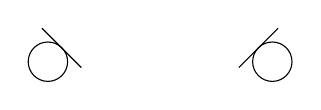
\begin{tikzpicture}[scale=1]
        \coordinate (Gesto) at (0,0);
        \campana{0}{-.3}{.8}{ordinaria}{libera}{Gesto}
     %   \draw (-2.25,-2.25) -- (-1.25,-1.25) -- (-1,-1.25) -- (-2,-2.25) -- cycle;
     %   \draw[rounded corners=2pt] (-2.25,-2.25) -- ++(+.75,+.75) -- ++(+.25,0) -- ++(-1,-1) -- cycle;
     %   \draw[rounded corners=2pt] (+2.25,-2.25) -- ++(-1,+1) -- ++(-.25,0) -- ++(+1,-1) -- cycle;
     \draw (-1.425,-1.425) circle[radius = .25cm];
     \draw (1.425,-1.425) circle[radius = .25cm];
     \draw (1,-1.5) -- ++(.5,.5)   ;
     \draw (-1,-1.5) -- ++(-.5,.5)   ;
    \end{tikzpicture}
\end{minipage}
\hfill
\begin{minipage}{0.75\textwidth}
        La microfonazione necessaria consiste in due microfoni a condensatore, non direzionali. Le loro capsule guardano il corpo della campana dal basso.
        Questa disposizione è necessaria poiché i due microfoni si sommeranno in ingresso al DSP per rafforzare il contributo simile in fase.
    \end{minipage}
\end{figure}

\null
\quad  % Aggiunge uno spazio fisso tra i minipage


\begin{center}
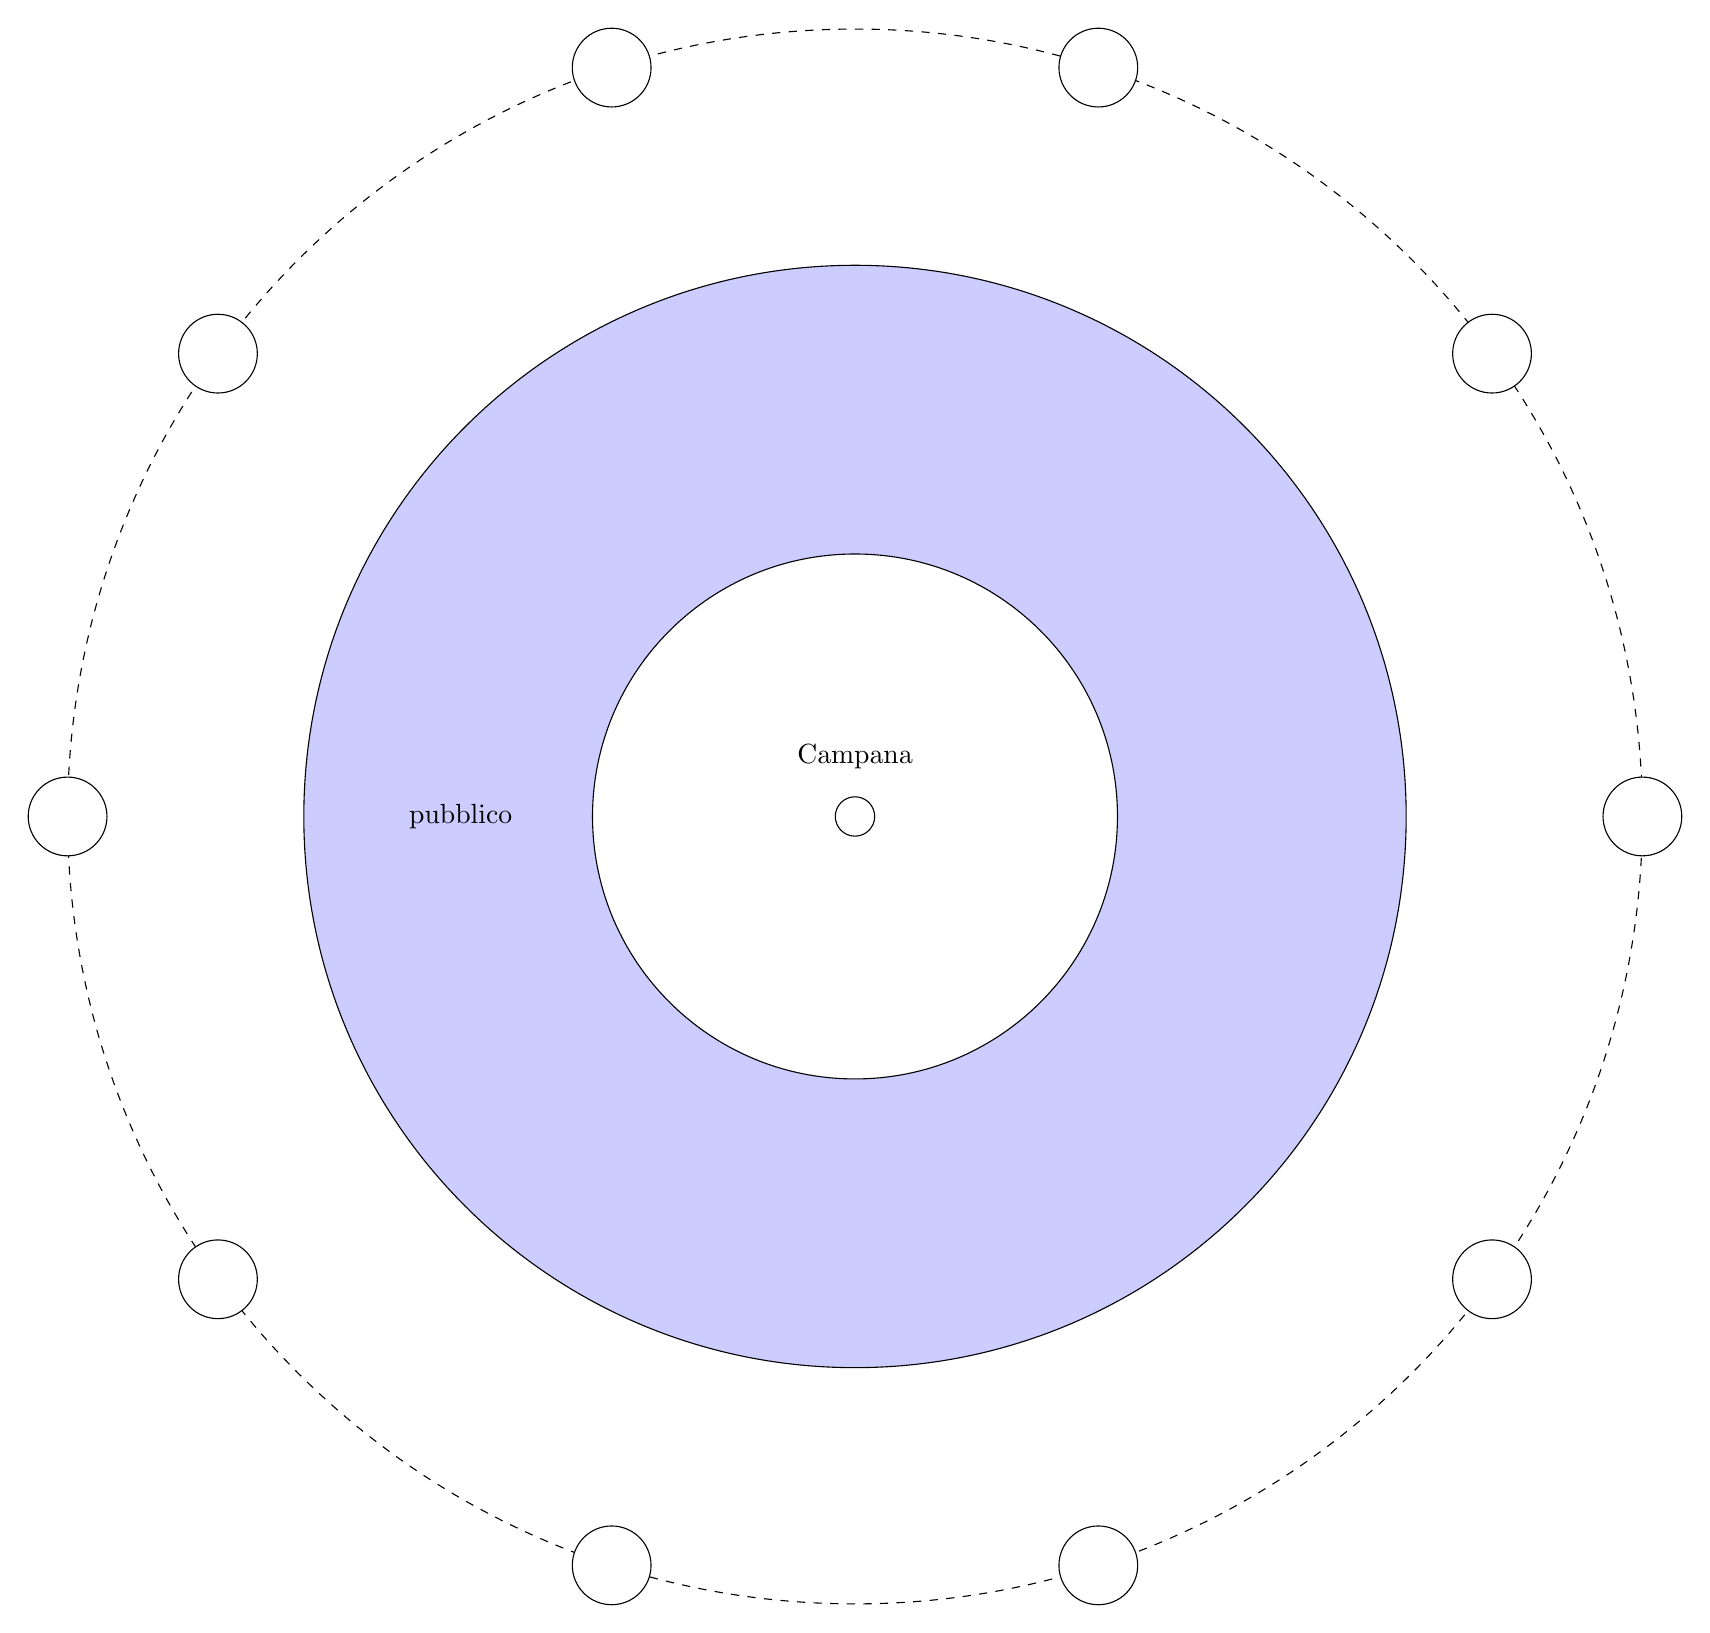
\begin{tikzpicture}[scale=1]
% Definisci le variabili
\def\radius{10cm}  % Raggio della circonferenza principale
\def\smallradius{0.5cm}  % Raggio dei cerchi piccoli
\def\n{10}  % Numero di cerchi

% Disegna la circonferenza principale (opzionale, commenta se non la vuoi visualizzare)
\draw [dashed] (0,0) circle (\radius);
\node[draw,circle,minimum size = \radius+4cm, inner sep=0pt,fill=blue!20] (pino) at (0,0) {};
\node[xshift=2cm] at (pino.west) {pubblico};
\draw [fill=white] (0,0) circle (\radius/3);

% Disegna i cerchi lungo la circonferenza
\foreach \i in {1,...,\n} {
    \node[draw,circle,fill=white,minimum size=2*\smallradius] 
        at ({360/\n * (\i - 1)}:\radius) {};
}
\coordinate (Gesto) at (0,0);
\node [draw,circle,minimum size = .5cm, inner sep=0pt] (camp) at (0,0) {};
\node[yshift=.5cm] at (camp.north) {Campana};

\end{tikzpicture}
\end{center}



\end{document}


